\scanpage{49}
\mspage{5)}

Cette opération de \unsure{somme|sommes} est la plus triviale parmi les opérations qu'il nous faudra expliciter et transcrire (combinatoirement) dans la suite. Notons de suite, pour $(X,\widetilde\Sigma,R)$\deleted{\unsure{,}} donné
\[
 X\,\deleted{\unsure{\ne}}\ \text{connexe}\quad\Longleftrightarrow\quad\Gamma MD(X,\widetilde\Sigma,R)\ \text{connexe}
\]
plus précisément
\[
 \pi_0(X)\simeq\pi_0(\Gamma MD(X,\widetilde\Sigma,R))
\]

% slanted
\margin{donner la formule pour le genre d'un $\alpha\in\pi_0(X)\simeq\pi_0(\Gamma)$ en termes de la pondération $g_s$ --- plus généralement, le \uline{genre total} est donné par $g=\sum_{s\in S}g_s+c(\Gamma)$}

% slanted
\margin{``indice de connexion'' du graphe $=\deleted{\unsure{\chi(\Gamma)}}\unsure{\mathrm{rg}}\ H_1(\Gamma)$}

\uline{Cas particuliers}.

a) Cas de $S_{*}{\unsure{\mathscr T|\mathbb T}}_{\mathrm{top}}^{\pm}$ \deleted{$\unsure{S\mathscr T_{\mathrm{top}}}$} --- \unsure{i.e.|ici|idem} $\Sigma=\varnothing,\ \widetilde\Sigma=\partial X$.

Cela \unsure{correspond} au cas des graphes $MD$ \deleted{qui} où \inserted{toutes les arêtes sont libres, i.e.,} tous les sommets sont isolés (sauf arêtes libres)

\deleted{Elle} \inserted{Ce graphe} est \deleted{une} déterminé par
\diagram{\begin{tikzcd}[ampersand replacement=\&,column sep=large]
 A\;(=\vec A=\vec A^\sigma)\arrow[d]\arrow[r,"r"] \& \mathbb N\\
 S\arrow[r,"\gamma"] \& \mathbb N
\end{tikzcd}}

Le cas de $\mathscr T_{\mathrm{top}}^{\pm}$ correspond à celui où $\rho=0$, donc la situation est donnée par
\diagram{\begin{tikzcd}[ampersand replacement=\&]
 A=A_0\arrow[d]\&\\
 S\arrow[r,"\gamma"]\&\mathbb N .
\end{tikzcd}}

\figure{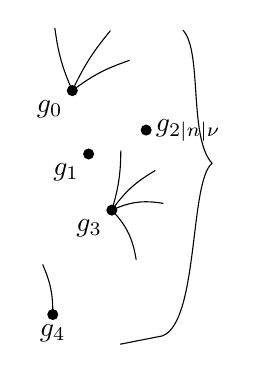
\begin{tikzpicture}[x=.67cm,y=.66cm,line cap=round]
\draw (.6,3.6) to[bend left=8](.27,4.8) (.6,3.6) to[bend left=7](1.32,4.75) (.6,3.6) to[bend left=9](1.68,4.18);
\fill (.6,3.6) circle (2pt) node[below left]{$g_0$};
\fill (.91,2.38) circle (2pt) node[below left]{$g_1$};
\fill (2.0,2.84) circle (2pt) node[right]{$g_{\unsure{2|n|\nu}}$};
\draw (1.35,1.3) to[bend right=8](1.52,2.44) (1.35,1.3) to[bend left=12](2.17,2.06)
 (1.35,1.3) to[bend left=17](2.32,1.43) (1.35,1.3) to[bend left=17](1.81,.35);
\fill (1.35,1.3) circle (2pt) node[below left]{$g_3$};
\draw (.23,-.71) to[bend right=12](.04,.25); \fill (.23,-.71) circle (2pt) node[below]{$g_4$};
\draw (2.7,4.76).. controls (3.07,4.35) and (2.8,2.7)..(3.25,2.2)
 .. controls (2.82,1.86) and (3,-.85)..(2.31,-1.12)--(1.51,-1.28);
\end{tikzpicture}}

\deleted{type $(g,\nu)$ d'une \unsure{surface}} Le cas d'une structure connexe ($\mathrm{card}.S=1$ \inserted{i.e. $S=\{s\}$}) est \deleted{\unsure{donné par la donnée}} \inserted{caractérisé par la donnée} des deux entiers $(g,\nu)$ \quad ($g=$ genre, $\nu={}$ nb de trous)
\[
 g=\gamma(s),\quad \nu=\mathrm{card}\,A
\]
% archive sheet number: 48

